\documentclass[12pt,notitlepage]{article}

% Overleaf project:
% https://www.overleaf.com/project/5fdb880ef955c3369964d601

% View-only link:
% https://www.overleaf.com/read/hkybwqtbtvjb


\usepackage{amsmath, amsfonts, amssymb}
\usepackage[svgnames]{xcolor}
\usepackage{datetime2}
\usepackage{epstopdf}
\usepackage[
	colorlinks=true, 
	citecolor={DarkRed}, urlcolor={DarkBlue}, linkcolor={DarkBlue},
]{hyperref}

% http://ctan.math.washington.edu/tex-archive/macros/latex/contrib/mhchem/mhchem.pdf
\usepackage[version=3]{mhchem}

\usepackage{fullpage}
\setlength{\parindent}{0cm}

\usepackage{graphicx}
\graphicspath{{../images/}}

% Tables
\usepackage{booktabs}
\usepackage{arydshln}

% For editing purposes:
%\usepackage[margin=10pt]{geometry}

% https://latex.org/forum/viewtopic.php?t=10456
\usepackage{titlesec}
\titleformat{\subsubsection}[runin]% runin puts it in the same paragraph
{\normalfont\bfseries}% formatting commands to apply to the whole heading
{\thesubsubsection}% the label and number
{}% space between label/number and subsection title
{}% formatting commands applied just to subsection title
[.]% punctuation or other commands following subsection title


\newcommand{\TODO}[1]{\textrm{\color{red}TODO: #1}}

% https://bitbucket.org/goodnightmath/covariance/src/master/tex/main.tex

%%%%%%%%%%%%%%%%%%%%%%%%%%%%%%%%%%%%%%%%%%%%%%%%%%%%%%%%%%%%%%%%%%%%%%%%%%%%%%%
% http://tex.stackexchange.com/a/106577/44073
\usepackage{ifthen}
\newcounter{todoindex}\setcounter{todoindex}{0}
\newcommand\ADDTODO[1]{%
	\addtocounter{todoindex}{1}%
	\expandafter\gdef\csname todo\roman{todoindex}\endcsname{#1}%
	%\expandafter\csname todolabel\roman{todoindex}\endcsname
	\label{todolabel\roman{todoindex}}
}
\renewcommand\TODO[1]{%
	{%
		\ADDTODO{#1}%
		{\textrm{\color{red}TODO(\arabic{todoindex}): #1}}%
	}%
}
\newcommand\CHECK[1]{%
	\ADDTODO{CHECK CLAIM: {#1}}%
	{\color{toverify}#1}%
	\smash{\marginnote{\text{\color{red}*}}}%
}
\newcounter{indextodo}
\newcommand{\SHOWTODOS}{%
	\setcounter{indextodo}{0}%
	\begin{enumerate}
	\item[{\color{red} TODOs:}]
	\whiledo{\value{indextodo} < \value{todoindex}}{%
		\addtocounter{indextodo}{1}%
		\item[\color{red}\arabic{indextodo}.]
		p.\pageref{todolabel\roman{indextodo}}.
		%
		\csname todo\roman{indextodo}\endcsname
	}%
	\end{enumerate}
}
%%%%%%%%%%%%%%%%%%%%%%%%%%%%%%%%%%%%%%%%%%%%%%%%%%%%%%%%%%%%%%%%%%%%%%%%%%%%%%%



\renewcommand{\d}{\mathrm{d}}

\newcommand{\TEXT}[1]{\quad\text{#1}\quad}
\newcommand{\with}{\text{ $:$ }}

\newcommand{\cbra}[1]{{\color{gray}\ensuremath{#1}}}
\newcommand{\signal}[1]{\ensuremath{\cbra{\langle}\mathrm{#1}\cbra{\rangle}}}
\newcommand{\protein}[1]{\ensuremath{\cbra{(}\mathrm{#1}\cbra{)}}}
\newcommand{\promoter}[1]{\ensuremath{\cbra{[}\mathrm{#1}\cbra{]}}}

% https://tex.stackexchange.com/questions/543953/arrow-with-blunted-end-head-in-math-mode
\newcommand{\act}{\ensuremath{\to}}
\newcommand{\rep}{\ensuremath{\mathrel{\raisebox{-.3ex}{\rotatebox{90}{\scalebox{1}[1.2]{$\bot$}}}}}}

\def\[#1\]{\begin{align}#1\end{align}}

% https://tex.stackexchange.com/questions/114113/how-to-label-text-with-equation-number
\newcommand{\eqnum}{\leavevmode\hfill\refstepcounter{equation}\textup{{(\theequation)}}}


\newcommand{\hh}[1]{{\color{Purple}#1}}
\newcommand{\ra}[1]{{\color{Blue}#1}}


\title{ibiocomp project}
\author{RA \& HH}
\date{\today}


\begin{document}

\maketitle




\section{Introduction}

\subsection{The game of 15 sticks}

Rules of the game:
%
\begin{quote}
	Two players start with 15 sticks
	and alternatingly 
	take 1, 2 or 3 sticks.
	\\
	The last to take a stick loses.
\end{quote}

\TODO{winning strategy, refer to Table \ref{t:logical-playera}}

\ra{[we may change the bibliography style later, but for the moment names are convenient]}

\subsection{General design}

\TODO{bit encoding}

\TODO{players and subtractor}

\TODO{signaling}

\TODO{mention tubes/microfluidics if applicable}

\TODO{manual intervention}


\section{Logical circuits}

\subsection{The players}

\TODO{Table \ref{t:logical-playera}}

% Generated in part using

% https://github.com/numpde/ibiocomp/blob/main/code/20201229_LogicalTables/PlayerA.py

% and
	
% https://crcit.net/c/205b0db18f954c4585b3f87d69fced6c
% https://crcit.net/c/84159c89986c4330978603aeace14aa1

% RA, 2020-12-30
	
\begin{table}[hpbt]
	\centering

	\begin{minipage}{0.3\linewidth}
		\centering
				
		Winning strategy:
		
		{\ }
		
		\begin{tabular}{cccc|c}
		\multicolumn{4}{c|}{Sticks left} & Take \\
		\hline
		15 & 11 & 7 & 3 & 2 \\
		14 & 10 & 6 & 2 & 1 \\	
		13 & 9  & 5 & 1 & 1 \\	
		12 & 8  & 4 &   & 3 \\	
		\end{tabular}
	\end{minipage}
	%
	\qquad
	%
	\begin{minipage}{0.25\linewidth}
		\centering
		\begin{tabular}{ccc|cc}
		\cee{w_A} &  \cee{s_1} &  \cee{s_0} &  \cee{r_1} &  \cee{r_0} \\
		\hline
		  0 &   0 &   0 &   0 &   0 \\
		  0 &   0 &   1 &   0 &   0 \\
		  0 &   1 &   0 &   0 &   0 \\
		  0 &   1 &   1 &   0 &   0 \\
		  1 &   0 &   0 &   1 &   1 \\
		  1 &   0 &   1 &   0 &   1 \\
		  1 &   1 &   0 &   0 &   1 \\
		  1 &   1 &   1 &   1 &   0 \\
		\end{tabular}
	\end{minipage}
	%
	\qquad
	%
	\begin{minipage}{0.3\textwidth}
		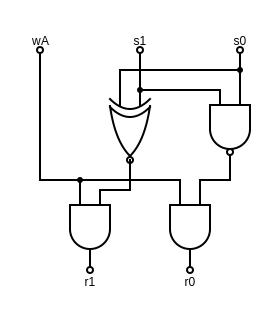
\includegraphics[width=\linewidth]{circuits/Logical-PlayerA}
	\end{minipage}
	
	\caption{%
		Logical circuit for {Player A}.
		%
		The input is a
		wake-up signal \cee{w_A}
		and the bits
		\cee{s_1}/\cee{s_0}
		of the current number of sticks
		(\cee{8 s_3 + 4 s_2 + 2 s_1 + s_0}).
		%
		The output is
		the number of sticks that 
		the player chooses to take,
		encoded as \cee{2 r_1 + r_0}.
		%
		Note that the output is cut off
		when \cee{w_A} is absent.
		%
		%
		The circuit for {Player B}
		is identical except
		that it is controlled up by \cee{w_B}.
	}
	
	\label{t:logical-playera}
\end{table}


\subsection{Subtractor}

\TODO{Table \ref{t:subtractor1}}

% Generated in part using
% https://github.com/numpde/ibiocomp/blob/main/code/20201229_LogicalTables/Subtractor.py

% RA, 2020-12-30

\begin{table}[hpbt]
\centering

\begin{minipage}{0.2\linewidth}
	\centering
			
	Half-subtractor:
	
	{\ }
	
	\begin{tabular}{cc|cc}
		\ce{s_3} &  \ce{c_3} &  \ce{d_3} &  -- \\
		\hdashline
		\ce{s_2} &  \ce{c_2} &  \ce{d_2} &  \ce{c_3} \\
		\hdashline
		\ce{s_0} &  \ce{r_0} &  \ce{d_0} &  \ce{c_1} \\
		\hline
         0 &          0 &          0 &          0 \\
         0 &          1 &          1 &          1 \\
         1 &          0 &          1 &          0 \\
         1 &          1 &          0 &          0 \\
	\end{tabular}
\end{minipage}
%
\quad
%
\begin{minipage}{0.3\linewidth}
	\centering
			
%		Full subtractor:
%		
%		{\ }
	
	\begin{tabular}{ccc|cc}
		\ce{s_1} &  \ce{r_1} &  \ce{c_1} &  \ce{d_1} &  \ce{c_2} \\
		\hline
         0 &          0 &          0 &          0 &          0 \\
         0 &          0 &          1 &          1 &          1 \\
         0 &          1 &          0 &          1 &          1 \\
         0 &          1 &          1 &          0 &          1 \\
         1 &          0 &          0 &          1 &          0 \\
         1 &          0 &          1 &          0 &          0 \\
         1 &          1 &          0 &          0 &          0 \\
         1 &          1 &          1 &          1 &          1 \\
	\end{tabular}
\end{minipage}
%
\quad
%
\begin{minipage}{0.3\linewidth}
	\begin{align*}
		\ce{& & 8 s_3 + 4 s_2 + 2 s_1 + s_0 &}
		\\
		- \ce{& & 2 r_1 + r_0 &}
		\\
		= \ce{& & 8 d_3 + 4 d_2 + 2 d_1 + d_0 &}
	\end{align*}
\end{minipage}

\caption{%
	The subtractor computes
	\ce{d = s - r} (mod 16).
	%
	Since \ce{r} only has 
	the two lowest bits, 
	a half-subtractor
	is sufficient for
	the bits \ce{d_0}/\ce{d_2}/\ce{d_3}
	and the carry flags \ce{c_1}/\ce{c_3},
	and
	only \ce{d_1}/\ce{c_2}
	require the full subtractor.
	%
	We have $\ce{d_0} = (\ce{s_0} \XOR \ce{r_0})$;
	$\ce{c_1} = \NOT (\ce{s_0} \geq \ce{r_0})$;
	$\ce{d_1} = ((\ce{s_1} + \ce{r_1} + \ce{c_1}) \mathbin{\mathrm{mod}} 2)$;
	$\ce{c_2} = \NOT (\ce{s_1} \geq \ce{r_1} \geq \ce{c_1})$.
	%
	See Fig.~\ref{f:logical-subtractor01}
	for a logic circuit of
	the subtractor.
}
\label{t:subtractor1}
\end{table}



\section{Genetic toolbox}


\TODO{mention 3-input boolean functions \cite{NielsenETAL2016}}

\TODO{ribocomputing OR and big AND gates \cite{GreenETAL2017}}

\TODO{Specify initial conditions}


\subsection{Transducers}


\subsubsection*{AmtR}

The TetR family member AmtR is 
the central regulator of nitrogen starvation response
in 
the Gram-positive bacterium
\emph{Corynebacterium glutamicum}
\cite{JakobyETAL2000}.
%
This repressor is released
by
the trimeric adenylylated $\mathrm{P_{II}}$-type 
signal-transduction protein GlnK
\cite{BeckersETAL2005, SevvanaETAL2017},
which is present upon
nitrogen starvation. 
%
The AmtR box and the regulon is 
characterized in 
\cite{BeckersETAL2005},
and
several variants are compared 
in \cite{MuhlETAL2009}.
%
%
\TODO{Do we need (to take care of) the GlnK release mechanism?}
%
It seems clear that 
AmtR sits on the DNA as a dimer
\cite{SevvanaETAL2017},
\cite[\S3.4.2]{Schwab2019}.
%
%
We therefore assume
the mechanism
\begin{subequations}
\[
	\cee{
		2 \protein{AmtR} + \promoter{AmtR}
		& <=>>
		\protein{AmtR}_2 \with \promoter{AmtR}
	}
	%
	\\
	%
	\cee{
		\promoter{AmtR} 
		& ->
		\promoter{AmtR} + \protein{Output}
	}
\]
\end{subequations}
and
the kinetics:
\begin{subequations}
\[
	\label{e:AmtR_Act}
	%
	\promoter{AmtR} 
	& =
	\frac{1}{1 + k_{\ref{e:AmtR_Act}} \protein{AmtR}^{n_{\ref{e:AmtR_Act}}}}
	\promoter{AmtR}_\text{total}
	%
	% here, k = forward / backward
	%
	,
	\\
	%
	\label{e:AmtR_Out}
	%
	\tfrac{\d}{\d{t}}
	\protein{Output} 
	& =
	k_{\ref{e:AmtR_Out}}
	\promoter{AmtR}
	.
\]
\end{subequations}
%
%

% Further literature
%\cite{MuhlETAL2009}
%\cite{BuchingerETAL2009}

\ra{working on this}


\subsubsection*{...}


\subsection{Sensors}

\TODO{Explain intercellular signaling pathways from \cite{DuETAL2020}}

\subsubsection*{3OC6-HSL/LuxR}

Pathway:
\[
	\signal{3OC6\text{-}HSL} \act \protein{LuxR} \act \promoter{Lux} \act \protein{Output}
	.
\]

 
The transcription activator \protein{LuxR}
occurs in Gram-negative bacteria
such as \emph{Vibrio fischeri}.
%
The bacterium is permeable to the (auto)inducer,
here \signal{3OC6\text{-}HSL}.
%
The inducer binds to the N-terminal of \protein{LuxR},
which otherwise inhibits its
functional C-terminal \cite{StevensDolanGreenberg1994}.
%
%
The purified C-terminal binds 
upstream of the \emph{lux} box 
(which is centered at $-42.5$bp \cite{EglandGreenberg1999});
however, 
together with the RNA Pol,
it protects the \emph{lux} box and the \emph{lux} operon
promoter
\cite{StevensDolanGreenberg1994}.
%
%
%
We abbreviate
$\protein{LuxR^\star} := \signal{3OC6\text{-}HSL} \with \protein{LuxR}$
and
$\promoter{Lux^\star} := \protein{LuxR^\star} \with \promoter{Lux}$.
%
%\TODO{
%Let $\protein{LuxR^\star}$ denote 
%the activated form
%$\signal{3OC6}:\protein{LuxR}$.
%}
%
%
We assume the mechanism:
%
\begin{subequations}
\[
	\cee{
		\signal{3OC6\text{-}HSL} + \protein{LuxR}
		& <=>>
		\protein{LuxR^\star}
	}
	\\
	\cee{
		\protein{LuxR^\star} + \promoter{Lux}
		& <=>>
		\promoter{Lux^\star}
	}
	\\
	\cee{
		\promoter{Lux^\star}
		& ->
		\promoter{Lux^\star} + \protein{Output}
	}
	.
\]
\end{subequations}
%
%=======
%	\protein{LuxR^\star} + \protein{RNApol} + \promoter{P_{Lux}}
%	& \longleftrightarrow
%	\protein{LuxR^\star} + \protein{RNApol} : \promoter{P_{Lux}}
%	\\
%	\protein{RNApol} : \promoter{P_{Lux}}
%	& \longrightarrow
%	\protein{RNApol} + \promoter{P_{Lux}} + \protein{Output}
%>>>>>>> c8a0f57bdb0a7b80747263819cbb64562e087765
%\TODO{
%\[
%	\signal{3OC6} + \protein{LuxR}
%	& \longleftrightarrow
%	\protein{LuxR^\star}
%	\\
%	\protein{LuxR^\star} + \protein{RNApol} + \promoter{Lux}
%	& \longleftrightarrow
%	\protein{LuxR^\star} + \protein{RNApol} : \promoter{Lux}
%	\\
%	\protein{RNApol} : \promoter{Lux}
%	& \longrightarrow
%	\protein{RNApol} + \promoter{Lux} + \protein{Output}
%\]
%}
% https://chem.libretexts.org/Bookshelves/Biological_Chemistry/Supplemental_Modules_(Biological_Chemistry)/Enzymes/Enzymatic_Kinetics/Sigmoid_Kinetics
%
%
%
and the kinetics:
%
\begin{subequations}
\[
	\label{e:LuxR_Act}
	%
	\protein{LuxR^\star} 
	& =
	\frac{
		\signal{3OC6\text{-}HSL}
	}{
		k_{\ref{e:LuxR_Act}} + \signal{3OC6\text{-}HSL}
	}
	\protein{LuxR}_\text{total}
%	\TEXT{initially}
%	\protein{LuxR^\star} = 0
	,
	%
	\\
	%%
	\label{e:P_Lux_Act}
	%
	\promoter{Lux^\star} 
	& =
	\frac{
		\protein{LuxR^\star}
	}{
		k_{\ref{e:P_Lux_Act}} + \protein{LuxR^\star}
	}
	\promoter{Lux}_\text{total}
%	\TEXT{initially}
%	\promoter{Lux^\star} = 0
	,
	%
	\\
	%
	\label{e:P_Lux_Out}
	%
	\tfrac{\d}{\d{t}}
	\protein{Output}
	& =
	k_{\ref{e:P_Lux_Out}} \promoter{Lux^\star}
	.
\]
\end{subequations}
%
%
In combination, we have
\[
	\tfrac{\d}{\d{t}}
	\protein{Output}
	=
	k_{\ref{e:P_Lux_Out}}
	\promoter{Lux}_\text{total}
	\frac{
		\signal{} \protein{}_\text{total}
	}{
		k_{\ref{e:LuxR_Act}} k_{\ref{e:P_Lux_Act}}
		+
		k_{\ref{e:P_Lux_Act}} \signal{}
		+
		\signal{} \protein{}_\text{total}
	}
	.
\]


\subsubsection*{Salicylate/NahR}

Pathway:
%
\[
	\signal{Sal} \act \protein{NahR} \act \promoter{Sal} \act \protein{Output}
	.
\]

%

According to 
\cite{SchellWender1986, HuangSchell1991},
the transcription activator \protein{NahR}
binds to the recognition site of \promoter{Sal} at
$-83$ to $-45$,
and does so without the inducer \cite[p.10837]{HuangSchell1991}.
The \protein{NahR} hence activate the expression of \promoter{Sal}.
%
%
%
In \cite{SchellBrownRaju1990},
it was suggested 
that the active configuration of \protein{NahR} is a tetramer,
while \cite{ParkLimShin2005}
reported that 
there could be three different complexes
%
$\protein{NahR} \with \promoter{Sal}$.

\TODO{make coherent}

\hh{
Nevertheless, the configuration changes 
then promotes the RNA polymerase binding near $-35$ (upstream of \promoter{Sal}).
%
%
The inducer
(here \signal{Sal}) can induce the conformation change of \protein{NahR},
and activates the promoter \promoter{Sal}.
}

%
%
Following \cite{Peking2013},
we suppose
that 
$4 \times \protein{NahR}$ bind to the DNA,
and
transcription starts
once
one $\signal{Sal}$
binds to each \protein{NahR}.
%
For the sensors we assume an abundance
of \protein{NahR}
\TODO{describe constitutive promoter},
hence the inactive form of the promoter
is $\protein{NahR}_4 \with \promoter{Sal}$.
%
%
We write
$
	\promoter{Sal^\star} :=
	\signal{Sal}_4 \with \protein{NahR}_4 \with \promoter{Sal}
$
for the active form.
%
%
We assume the mechanism
%
\begin{subequations}
\[
	\cee{
		\signal{Sal} + 
		\signal{Sal}_{k - 1} \with \protein{NahR}_4 \with \promoter{Sal}
		& <=>>
		\signal{Sal}_k \with \protein{NahR}_4 \with \promoter{Sal}
	}
	,
	\quad \text{k} = 1, 2, 3, 4,
	%
	%
	\\
	%
	%
	\cee{
		\promoter{Sal^\star}
		&
		->
		\promoter{Sal^\star} + \protein{Output}
	}
\]
\end{subequations}
%
%Mechanism (here \protein{NahR^\star} denotes the activated (tetramer) form):
%\[
%	\signal{Sal} + \protein{NahR}
%	& \longleftrightarrow
%	\protein{NahR^\star}
%	 \\
%	 \protein{NahR^\star} + \protein{RNApol} + \promoter{P_{Sal}}
%	& \longleftrightarrow
%	\protein{NahR^\star} + \protein{RNApol} : \promoter{P_{Sal}}
%	\\
%	\protein{RNApol} : \promoter{P_{Sal}}
%	& \longrightarrow
%	\protein{RNApol} + \promoter{P_{Sal}} + \protein{Output}
%	.
%\]
%
%
which we implement as:
%
\begin{subequations}
\[
	\label{e:NahR_Act}
	%
	\promoter{Sal^\star}
	& =
	\frac{
		\signal{}^{n_{\ref{e:NahR_Act}}}
	}{
		k_{\ref{e:NahR_Act}} + \signal{}^{n_{\ref{e:NahR_Act}}}
	}
	\promoter{Sal}_\text{total}
	,
	%
	%
	\\
	%
	%
	\label{e:NahR_Out}
	%
	\tfrac{\d}{\d{t}}
	\protein{Output}
	& =
	k_{\ref{e:NahR_Out}} 
	\promoter{Sal^\star}
	.
\]
\end{subequations}



\subsubsection*{pC-HSL/rpaR}

Pathway:
%
\[
	\signal{pC} \act \protein{RpaR} \act \promoter{rpa}
	\act 
	\protein{Output}
	.
\]

\hh{
The p-coumaroyl-HSL -- RpaR system 
(\signal{pC\text{-}HSL})
works similarly to AHL/LuxR
\TODO{use `protein`?}.
%
However, as they come from an anoxygenic phototrophic soil bacterium strain, 
the luxIR-type pair, rpaI and rpaR shows good orthogonality to many
QS signals in use \cite{SchaeferETAL2008}.
}

\ra{
The \emph{Rhodopseudomonas palustris} transcriptional regulator
\protein{RpaR},
when purified,
binds an inverted repeat element 
centered at $-48.5$bp
of its promoter
\cite{HirakawaETAL2011}.
%
%
Transcription depends on 
the inducer 
\emph{p}-coumaroyl-homoserine lactone,
or \signal{pC} for short.
%
%
%There is
%pC-HSL-RpaR-activated antisense transcription of \protein{rpaR}.
%
%
The complex 
$\signal{pC} : \protein{RpaR}$
bound to the promoter
activates transcription
\cite[Discussion]{HirakawaETAL2011}.
}


\subsubsection*{XX}



\subsubsection*{XX}

\ra{--}

\subsubsection*{XX}



\subsubsection*{XX}




\subsection{Recombinases}

\subsubsection*{Bxb1 integrase}

\TODO{``recombinase addressable data'' from \cite{BonnetSubsoontornEndy2012}}

\subsubsection*{XX}


\subsubsection*{XX}



\section{Discussion}

\TODO{risks}


\footnotesize
\bibliographystyle{apalike}
\bibliography{refs}

\SHOWTODOS

\leavevmode\vfill{\tiny\color{lightgray}\hfill{\DTMnow}}
\end{document}





